\documentclass[12pt,a4paper,titlepage,openany]{report}
\usepackage{zakljucna_FAMNIT_1_stopnja_MA_MEF_2016}

% Glava dokumenta:

\fancyhf{}
\lhead[]{{\fontsize{9.3}{12}\selectfont
Priimek I. Naslov zaključne naloge.\\
\noindent Univerza na Primorskem, Fakulteta za matematiko, naravoslovje in informacijske tehnologije, leto}}
\chead[]{\fancyplain{}{}}
\rhead[]{\fancyplain{\thepage}
{\thepage}}
\cfoot[]{\fancyplain{}{}}
\lfoot[]{\fancyplain{}{}}
\rfoot[]{\fancyplain{}{}}
\normalsize

%%%%%%%%%%%%%%%%%%%%%%%%% ZAČETEK DOKUMENTA %%%%%%%%%%%%%%%%%%%%%%%%%%%%%%%%%%%%%%%%%%5

%%%%%%%%%%%%%%%%%%%%%%%%% Naslovna stran %%%%%%%%%%%%%%%%%%%%%%%%%


\begin{document}
\pagenumbering{Roman}
\pagestyle{empty}
\begin{center}
\noindent \large UNIVERZA NA PRIMORSKEM\\
\large FAKULTETA ZA MATEMATIKO, NARAVOSLOVJE IN\\
INFORMACIJSKE TEHNOLOGIJE


\normalsize
\vspace{6cm}
Zaključna naloga\\
\textbf{\large Nadzor porabe električne energije z namensko razvitim merilcem in  spletnim portalom}\\
\normalsize
(Control of electrical usage with dedicated measurer and  web portal)\\
\end{center}

\begin{flushleft}
\vspace{5cm}
\noindent Boštjan Vižintin:
% v zgornjo vrstico dopišite ime in priimek študenta
\\
\noindent Računalništvo in informatika:
% v zgornjo vrstico dopišite ime študijskega programa
\\
\noindent Tatjana Zrimec:
% v zgornjo vrstico dopišite akademski naziv, ime in priimek mentorja
\\
%\noindent Somentor:
% če imate somentorja, v zgornjo vrstico dopišite akademski naziv, ime in priimek somentorja
% če somentorja nimate, zbrišite zgornjo in spodnjo vrstico
%\\
\end{flushleft}

\vspace{4cm}
\begin{center}
\large \textbf{Koper, Avgust 2016}
% dopišite mesec in leto oddaje zaključne naloge
\end{center}
\newpage

\pagestyle{fancy}
%%%%%%%%%%%%%%%%%%%%%%%%%%%%%%% Ključna dokumentacijska informacija (slo in ang) %%%%%%%%%%%

\section*{Ključna dokumentacijska informacija}

\medskip
\begin{center}
\fbox{\parbox{\linewidth}{
\vspace{0.2cm}
\noindent
Ime in PRIIMEK:\vspace{0.5cm}\\
Naslov zaključne naloge:\vspace{0.5cm}\\
Kraj:\vspace{0.5cm}\\
Leto:\vspace{0.5cm}\\
Število listov: \hspace{2cm} Število slik: \hspace{2.6cm} Število tabel:\hspace{2cm}\vspace{0.5cm}\\
Število prilog: \hspace{1.9cm} Število strani prilog: \hspace{1cm} Število referenc:\vspace{0.5cm}\\
Mentor:\vspace{0.5cm}\\
Somentor:\vspace{0.5cm}\\
Ključne besede:\vspace{0.5cm}\\
Math.~Subj.~Class.~(2010):\vspace{0.5cm}\\
{\bf Izvleček:}\\
Izvleček predstavlja kratek, a jedrnat prikaz vsebine naloge. V največ 250 besedah nakažemo problem, metode, rezultate, ključne ugotovitve in njihov pomen.
\vspace{0.2cm}
}}
\end{center}

\newpage

\section*{Key words documentation}

\medskip

\begin{center}
\fbox{\parbox{\linewidth}{
\vspace{0.2cm}
\noindent
Name and SURNAME:\vspace{0.5cm}\\
Title of final project paper:\vspace{0.5cm}\\
Place:\vspace{0.5cm}\\
Year:\vspace{0.5cm}\\
Number of pages:\hspace{1.6cm} Number of figures:\hspace{2.2cm} Number of tables:\vspace{0.5cm}\\
Number of appendices:\hspace{0.6cm} Number of appendix pages:\hspace{0.8cm}Number of references:\vspace{0.5cm}\\
Mentor: title~First Name~Last Name, PhD\vspace{0.5cm}\\
% opomba: za "title" vpišite eno od naslednjega:
% Assist.~Prof. (če je naziv docent),
% Assoc.~Prof. (če je naziv izredni profesor),
% Prof. (če je naziv profesor)
Co-Mentor:\vspace{0.5cm}\\
Keywords:\vspace{0.5cm}\\
Math.~Subj.~Class.~(2010):\vspace{0.5cm}\\
{\bf Abstract:}
\vspace{0.2cm}
}}
\end{center}




%%%%%%%%%%%%%%%%%%%%%%%%%%%%%%% Zahvala %%%%%%%%%%%%%%%%%%%%%%%%%%%%%%%%%%%%%

\newpage
\section*{Zahvala}


Tu se zahvalimo sodelujočim pri zaključni nalogi, osebam ali ustanovam, ki so nam pri delu pomagale ali so delo omogočile. Zahvalimo se lahko tudi mentorju in morebitnemu somentorju.

%%%%%%%%%%%%%%%%%%%%%%%%%%%%% Kazala %%%%%%%%%%%%%%%%%%%%%%%%%%%%%%
\newpage

% Dodamo kazala (po potrebi):
\tableofcontents
\addtocontents{toc}{\protect\thispagestyle{fancy}}
\newpage
\listoftables
\addtocontents{lot}{\protect\thispagestyle{fancy}}
\newpage
\listoffigures
\addtocontents{lof}{\protect\thispagestyle{fancy}}
\newpage
% ker priloge niso oštevilčene, tudi pikic do številk strani (ki jih ni) ne izpišemo
\renewcommand{\cftdot}{}
\listofappendices
\thispagestyle{fancy}
\newpage

\chapter*{Seznam kratic}
\thispagestyle{fancyplain}
\begin{longtable}{@{}p{1cm}@{}p{\dimexpr\textwidth-1cm\relax}@{}}
\nomenclature{$tj.$}{to je}
\nomenclature{$npr.$}{na primer}
\end{longtable}
\newpage

\normalsize

%%%%%%%%%%%%%%%%%%%%%%%%%%%%%%%%%% Poglavja: %%%%%%%%%%%%%%%%%%%%%%%%%%%%%%%%%%%%%

% Namig: Za večjo preglednost datoteke lahko vsebino vsakega poglavja shranite v poseben .tex dokument
% v isto mapo, kjer je shranjena osnovna .tex datoteka. Nato poglavja vstavite v dokument s klicem \include
% Primer: PrvoPoglavje.tex in DrugoPoglavje.tex vstavimo tako:
% \include{PrvoPoglavje}
% \include{DrugoPoglavje}

\chapter{Uvod}
\thispagestyle{fancy}
\pagenumbering{arabic}

Tu opišemo problem, ki ga v zaključni nalogi obravnavamo. Predstavimo osnovne ideje in uvedemo
osnovne definicije in oznake. V uvodu lahko tudi povzamemo matematična dejstva, ki jih bomo
kasneje uporabili. Citiramo literaturo, ki je relevantna za obravnavane pojme, lahko tudi dodatno literaturo.

\chapter{Definicija problema}
\thispagestyle{fancy}
\pagenumbering{arabic}

Poraba električne energije v gospodinjstvih narašča in je v letu 2010 znašala približno 3.5 kWh na povprečno gospodinjstvo. Narašča tudi delež gospodinjstev opremljenih z dobrinami, ki za svoje delovanje potrebujejo elektriko. Na primer pomivalni stroj, stroj za sušenje perila, mobilni telefon, CD naprave, mikrovalovna pečica ter osebni računalnik. Kljub izboljšanju energetske učinkovitosti nekaterih naprav se poraba elektrike v povprečju ne znižuje, saj število naprav v gospodinjstvih narašča. Ker gospodinjstva porabijo tretjino skupne električne energije(http://shrinkthatfootprint.com/how-do-we-use-electricity), bi lahko z majhno spremembo porabe v posameznih gpospodinjstvih veliko vplivali na skupno porabo električne energije. Gospodinjstva redno prejemajo račune za količino porabljene električne energije vendar uporabniku skupna poraba električne energije ne koristi pri predstavi, kje v gospodijstvu bi lahko porabo omejil. Ideja je torej načrtovati in izdelati tak sistem, ki bi uporabnikom omogočal natančnejši nadzor porabe električne energije in s tem prikazal možnosti zmanjšanja električne energije.

\chapter{Rešitev problema}
\thispagestyle{fancy}
\pagenumbering{arabic}

Porabo električne energije v gospodinjstvih lahko zmanjšamo, vendar je to veliko enostavneje, če imamo natančen vpogled v porabo posameznih električnih naprav, ki si jih lasti gospodinjstvo. Glavna funkcija sistema bi torej bila nadzor porabe električne energije. Uporabniki bi lahko sami določili merilne točke in tako natačno izmerili porabo električne energije na posameznih merilnih mestih. Točna poraba bi bila nato prikazana za posamezna merilna mesta v obliki grafa. Poleg nadzora porabe, bi si lahko uporabniki določili različna opozorila. Sistem bi jih glede na opozorila opozarjal na preveliko uporabo oziroma na prekoračitev porabe električne energije in imel možnosti izklopa porabnikov v primeru sprožitve opozorila. Za lažjo predstavo o količini porabljene električne energije bi sistem omogočal tudi primerjavo porabe električne energije med seboj podobnimi gospodinjstvi.

\chapter{Težave}
\thispagestyle{fancy}
\pagenumbering{arabic}

Ena od težav, ki nastopi pri merjenju porabe električne energije je montaža merilcev. Ker povprečno gospodinjstvo ne obvlada elektronike, bi morali biti merilci enostavni za montažo, sicer bi vsako montažo moral opraviti strokovnjak kar bi povečalo stroške in tako odvrnilo zanimanje s strani uporabnikov. Težave nastopijo tudi zaradi velike količine podatkov, ki jih merilne naprave konstantno pošiljajo na strežnik. 

\chapter{Ekonomska izvedljivost}
\thispagestyle{fancy}
\pagenumbering{arabic}

Ena od omenjenih težav je velika količina podatkov ki se konstantno pošilja na strežnik, kar pomeni da bi strežnik moral biti zelo zanesljiv, saj igra ključno vlogo v sistemu. Taki strežniki lahko predstavljajo velik strošek, zato je nujno potreben nekakšen prihodek s strani uporabnikov sistema. Sistem bi zato omogočal prosto verzijo in plačljivo verzijo, katera nebi imela nekaterih omejitev ki bi jih imela prosta verzija. 
Poleg strežnika je potrebno načrtovanje in izdelava merilcev, za kar bi potrebovali nekaj začetnega kapitala. 
Pri izdelavi prototipa merilca in spletne aplikacije za diplomsko nalogo so stroški zanemarljivi, saj bomo za izdelavo merilca uporabili razvijalno ploščico arduino, ter njemu kompatibilne senzorje, za strežnik pa bo zadostoval navaden osebni računalnik.

\chapter{Analiza in definiranje zahtev}
\thispagestyle{fancy}
\pagenumbering{arabic}

Sistem za nadzor porabe električne energije bo na voljo vsem uporabnikom, ki bi želeli natančnejši pogled svoje porabe električne energije in tako potencialno zmanjšati porabo, kjer je to le možno. Sistem bo podpiral dve vrsti uporabnikov:
\begin{itemize}
\item Proste uporabnike
\item Plačljive uporabnike
\end{itemize}
Funkcije sistema bodo enake za vse uporabnike z razliko, da bodo imeli prosti uporabniki nekaj omejitev pri nekaterih funkcijah kot na primer:
\begin{itemize}
\item Omejeno število meritev posameznega merilnega mesta na dan (manj natančna poraba)
\item Omejeno število dni hranjenja starih meritev
\item Omejeno število merilnih mest
\item Omejeno število nastavljivih opozoril
\end{itemize}


\section{Funkcijske zahteve}
\thispagestyle{fancy}
\pagenumbering{arabic}

\subsection{Funkcijske zahteve sistema:}
\begin{itemize}

\item Registracija uporabnika v sistem
\item Prijava uporabnika v sistem
\item Nadgradnja uporabnika v plačljivega uporabnika
\item Vnos novega merilca
\item Urejanje vnešenih merilcev
\item Imenovanje posameznih merilnih mest že vnešenih merilcev
\item Urejanje že vnesenih merilnih mest
\item Dodajanje novih opozoril
\item Urejanje že vnesenih opozoril
\item Pregled porabe električne energije po merilnih mestih z možnostjo različnih filtrov
\item Pogled porabe posameznega senzorja "v živo"
\item Pregled napak senzorja/sistema
\item Pregled navodil za uporabo
\item Nastavitev stikal za vklop/izklop merilnih mest/porabnikov

\end{itemize}

\subsection{Prijava/registracija v sistem:}
Kot večina aplikacij, bo sistem omogočal uporabnikom registracijo in nato prijavo v sistem. Poleg prijave in registracije bodo uporabniki imeli možnost nadgradnje svojega računa in si s tem omgočili dodatne funkcije sistema, ki ne bodo mogoče navadnim uporabnikom.

\subsection{Vnos in urejanje novega merilca:}
Uporabniki bodo za merjenje potrebovali posebne merilce, razvite točno za ta namen, katere bo mogoče kupiti. Merilci bojo med seboj ločeni s posebnim nizem znakov, ki bo vnaprej določen in ga bo moral uporabnik vnesti v sistem ob vnosu novega merilca. Merilcu bo uporabnik ob vnosu v sistem določil še ime in število merilnih mest. Že vnesenim merilcem bo lahko uporabnik spremenil ime in število merilnih mest.

\subsection{Imenovanje in urejanje merilnih mest:}
Uporabiki bodo morali pred začetkom opravljanja meritev, imenovati merilne točke. Vsaka točka bo imela svoje ime in pod ime. Merilna mesta, ki bodo merila na primer vsako vtičnico posebej bodo imela enako ime ampak različno pod ime. Imena bo mogoče tudi spremeniti.

\subsection{Dodajanje in urejanje opozoril:}
Uporabniki bodo lahko izbirali med dvema vrstama opozoril:
\begin{itemize}
\item Ko bo trenutna poraba večja od določene vrednosti, ki jo bo določil uporabnik
\item Ko bo skupna poraba na merilnem mestu presegla vrednost, ki jo bo določil uporabnik.
\end{itemize}
Uporabnik bo določil ime, tip, obdobje in vrednost opozorila. Ko bo sistem zaznal da je neka vrednost presegla vrednost opozorila, bo o tem obvestil uporabnika (v obliki e-mail sporočila). Uporabniku bo ob prihodu na stran z opozorili prikazano katera opozorila so presegla vrednost.
Ko se bodo opozorila sprožila bodo postala neaktivna. Uporabnik bo lahko ta opozorila, vključno z ostalimi urejal (spreminjal imena, vrednosti in jih ponovno aktiviral).

\subsection{Pregled porabe električne energije:}
Uporabnik bo lahko za vsako merilno mesto pregledal porabo v obliki grafa. Podatke bo mogoče filtrirati po merilnih mestih. Mogoč bo tudi prikaz večjih merilnih mest skupaj. Meritve bodo prikazane v trenutni porabi za določen čas ali pa v skupni porabi.

\subsection{Pregled porabe "v živo":}

\subsection{Pregled napak:}

\subsection{Pregled navodil:}

\subsection{Nastavitev stikal za vklop/izklop merilnih mest/porabnikov:}

\chapter{Načrtovanje merilnega sistema - Komponent}
\thispagestyle{fancy}
\pagenumbering{arabic}

\section{Arduino}
Arduino je odprtokodna elektronska platforma zgrajena z hardwerom in softwerom ki je lahek za uporabo. Nastal je na inštitutu Ivrea Interaction Design, kot orodje za hitro izdelavo prototipov, namenjen pa je bil za študente brez predhodnega znanja elektrotehnike in programiranja. Kmalu za tem je postal zelo priljubljen in posledično se je začel razvijat. Zmore od enostavnih projektov kot so aktivacija motorja, prižiganje luči, branje senzorja pa do 3D printanja in uporabo v vgrajenih sistemih, uporabljajo ga pa tako začetniki kot tudi profesionalci. Na voljo je več verzij Arduinota, ki pa se razlikujejo predvsem v verziji mikrokontrolerja od katerega je tudi odvisno številov digitalnih in analognih vhodov in izhodov ter ceni, ki znaša od od 20 do 80 evrov. Ker je platforma kot že omenjeno odprtokodna pa seveda lahko dobimo Arduino ploščice pod drugim imenom, z enako funkcionalnostjo za veliko ceneje. Zaradi cene, razširjene uporabe platforme in obsežne dokumentacije, ki je na voljo na spletu, je bil Arduino kandidat za izdelavo naprave za diplomsko nalogo. Kasneje se je izkazalo, da je Raspberry pi nekoliko bolj     primeren.

\section{Raspberry Pi}
Kot že omenjeni Arduino je bil Raspberry Pi namenjen promoviranju in učenju osnov računalništva. Vsi modeli Raspberry Pi vsebujejo Broadcom-ov Soc(System on a chip), kateri je zgrajen iz ARM-ovega procesorja (CPU) in grafičnega procesorja GPU. Ure procesorjev so med 700MHz in 1.2GHz, pomnilnik pa varira med 256MB in 1GB RAM. Za shrambo operacijskega sistema je uporabljena Secure Digital (SD) kartica različnih velikosti. Večina ploščic ima med 1 in 4 USB vhodov, HDMI in composit video izhod, 3.5mm audio jack. Nižje razredni vhodi/izhodi so na voljo preko številnih GPIO pinov, ki podpirajo protokole kot na primer I2C. Nekatere ploščice imajo tudi Ethernet port in WIFI ter bluetooth. Deluje na operacijskem sistemu raspbian, ki je Debianova različica linuxove distribucije.

\section{Arduino ali Raspberry Pi}
Za razvoj merilnika za naše potrebe, razvojna ploščica Arduino zadostuje vsem zahtevam, zato je bila prva verzija merilnega instrumenta izdelana z Arduino ploščico verzijo Arduino UNO. Arduino je s pomočjo senzorjev uspešno opravljal meritve, vendar je bil nestabilen in sicer pri večkratnem zaporednem pošiljanju requestov na strežnik  je "zmrznil". Ker težave nismo uspeli odpraviti smo zato Arduino zamenjali z Raspberry Pi. Raspberry Pi se je izkazal enostavnejši za uporabo ( naprednejši jezik???? ), vendar smo pri zamenjavi naleteli na novo težavo in sicer Raspberry Pi nima analognih vhodov ( Arduino ima vgrajene analogno digitalne pretvornike na ploščici). Problem smo rešili z uporabo analogno/digitalnega pretvornika MCP3008.

\section{Analogno digitalni pretvornik MCP3008}
MCP3008 je nizkocenovni 8 kanalni 10 bitni analogno digitalni pretvornik. Natančnost tega čipa je podobna čipu uporabljenem na Arduino UNO. V primeru da bi kasneje želeli natančnejše meritve bi morali ta čip zamenjati za natančnejši čip na primer: ADS1015(12 bit) ali še natančnejši ADS1115(16 bit). Komunikacija med Raspberry Pi in MCP3008 poteka po SPI protokolu.

\section{SPI}
SPI(ang. Serial Peripheral Interface bus) je standard za sinhrono serijsko podatkovno povezavo, ki je uporabljena za kratke povezave. Najpogosteje je uporabljena v vgrajenih sistemih. Standard je bil razvit leta 1980, razvila pa ga je Motorola. Kmalu za tem je postal "de facto" standard. Tipično uporabo SPI vodila lahko zasledimo pri Secure Digital karticah (SD) in pri LCD zaslonih. Naprave ki uporabljajo SPI protokol, komunicirajo med seboj v dvosmernem načinu(full duplex), s principom nadrejenega/podrejenega(master/slave), z enim nadrejenim(master) in možnostjo več podrejenih(slave), katere nadrejeni izbira preko SS vodila. Včasih SPI-ju rečemo kar štiri žično serijsko vodilo, ker za svojo delovanje uporablja štiri žice.

\begin{itemize}
\item MOSI: MOSI priklop je uporabljen za prenos podatkov iz SPI modula, ko je nastavljen kot nadrejeni in za sprejem podatkov ko je nastavljen kot podrejeni.
\item MISO: MISO priklop je uporabljen za prenos podatkov iz SPI modula, ko je nastavljen kot podrejeni in za sprejem podatkov ko je nastavljenkot nadrejeni.
\item SS: This pin is used to output the select signal from the SPI module to another peripheral with which a data transfer is to take place when its configured as a Masterand its used as an input to receive the slave select signal when the SPI is configured as Slave.
\item SCK: SCK priklop je uporabljen za izhod urinega signala, kateri določa takt prenosa podatkov med nadrejenim/podrejenim.
\end{itemize}

\section{Metode merjenja toka}
Zazanavanje toka je uporabljeno za izvajanje dveh poglavitih funkcij. Meri se količina toka, ki teče skozi porabnik, kar lahko uporabimo za nadzor porabe in meri se previsok tok oziroma napake. Če tok preseže varne meje, programska ali strojna oprema lahko ustrezno reagira in izklopi delovanje naprave. Za opravljanje meritev toka poznamo veliko načinov:

\begin{itemize}
\item Resistive (direktno merjenje)

\begin{itemize}
\item Current sense resistors
\end{itemize}

 \item Magnetno (indirektno merjenje)

\begin{itemize}
\item Current transformer
\item Rogowski coil
\item Hall effect device
\end{itemize}

\item Transistor (direktno merjenje)

\begin{itemize}
\item RDS(ON)
\item Ratio-metric
\end{itemize}

\end{itemize}

Vsaka od metod merjenja ima prednosti in slabosti, ki so ključne ko izbiramo metodo in vrsto zenzorja, ki ga bomo uporabili
v naši aplikaciji. Metode merjenja so razdeljene v dve glavne kategorije: direktno merjenje in indirektno merjenje.
Direktno merjenje pomeni, da je senzor oziroma naprava za merjenje toka priključena direkno na izvor pod napetostjo, 
indirektno merjenje pa pomeni, da je senzor oziroma naprava za merjenje toka nekako ločena od izvora napetosti, 
kar je lahko ključno za varnost aplikacije.

\subsection{Resistive}
\subsubsection{Current Sense Resistor}
The resistor is a direct method of current measurement that has the benefit of simplicity and linearity. The current sense resistor
is placed in line with the current being measured and the resultant current flow causes a small amount of power to be converted
into heat. This power conversion is what provides the voltage signal. Other than the favorable characteristics of simplicity and
linearity, the current sense resistor is a cost-effective solution with a stable temperature coefficient of resistance (TCR) of
< 100 ppm or 0.01  and does not suffer the potential of avalanche multiplication or thermal runaway. Additionally,
low-resistance (< 1 m is available) metal alloy current sense products offer superior surge performance for reliable protection
during short circuit and overcurrent events.

\subsection{Magnetic}
\subsubsection{Current Transformer}
A current transformer (Fig. 1) provides three key advantages: isolation from line voltage; lossless current measurement; and a
large signal voltage that can provide noise immunity. This indirect current measurement method requires a changing current -
such as an AC, transient current, or switched DC - to provide a changing magnetic field that is magnetically coupled into the
secondary windings. The secondary measurement voltage can be scaled according to the turns ratio between the primary and
secondary windings. This measurement method is considered “lossless” because the circuit current passes through the copper
windings with very little resistive losses (Fig. 2). However, a small amount of power is lost due to transformer losses from the
burden resistor, core losses, and primary and secondary DC resistance.

\subsubsection{Rogowski Coil}
The Rogowski coil (Fig. 3) is similar to a current transformer in that a voltage is induced into a secondary coil that is proportional
to the current flow through an isolated conductor. The difference is that the Rogowski coil is an air core design as opposed to
the current transformer that relies upon a high-permeability core, such as a laminated steel, to magnetically couple to a
secondary winding. The air core design has a lower inductance to provide a faster signal response and very linear signal voltage.
Because of its design, it is often used as a temporary current measurement method on existing wiring such as a handheld meter.
This could be considered a lower-cost alternative to the current transformer.

\subsubsection{Hall Effect}
When a current-carrying conductor is placed in a magnetic field (Fig. 4), a difference in potential occurs perpendicular to the
magnetic field and the direction of current flow. This potential is proportional to the magnitude of the current flow. When there
is no magnetic field and current flow exists, then there is no difference in potential. However, when a magnetic field and current
flow exist, the charges interact with the magnetic field causing the current distribution to change, which creates the hall voltage
(Fig. 5).
The advantage of hall effect devices is that they are capable of measuring large currents with low power dissipation. However,
there are numerous drawbacks that can limit their use, such as non-linear temperature drift requiring compensation, limited
bandwidth, low-range current detection requiring a large offset voltage that can lead to error, susceptibility to external magnetic
fields, ESD sensitivity, and high cost.

\subsection{Transistor}
\subsubsection{RDS(ON) - Drain-to-Source On-Resistance}
Transistors are considered a “lossless” overcurrent detection method since they are standard control components to the circuit
design and no further resistance or power dissipating devices are required to provide a control signal. Transistor datasheets
provide the on-resistance for the drain-to-source (RDS(ON)) with a typical resistance in the m range for power MOSFETs. This
resistance consists of several components that begin with the leads (Fig. 6) connecting to the semiconductor die through the
resistance that makes up the numerous channel characteristics. Based on this information, the current passing through the
MOSFET can be determined by ILoad = VRDS(ON) / RDS(ON).
Each constituent of the RDS(ON) contributes to measurement errors that are due to minor variations in the resistances of the
interface regions and TCR effects. The TCR effects can be partially compensated by measuring temperature and correcting the
measured voltage with anticipated changes in resistance due to temperature. Often times the TCR for MOSFETs can be as large
as 4000 ppm, which is equivalent to a 40  change in resistance for a 100  rise. Generally, this measurement method
provides a signal with approximately 10  to 20  accuracy. Depending on the accuracy requirements, this may be an
acceptable range for providing overcurrent protection.

\subsection{Ratio Metric - Current Sense MOSFETs}
The MOSFET consists of thousands of parallel transistor cells that reduce the on-resistance. The current sensing MOSFET uses
a small portion of the parallel cells and connects to the common gate and drain, but a separate source (Fig. 7). This creates a
second isolated transistor; a “sense” transistor. When the transistor is turned on, the current through the sense transistor will
be a ratio comparable to the main current through the other cells.
Depending on the transistor product, the accuracy tolerance range can vary from as low as 5  to as wide as 15  or 20 .
This is generally not suitable for current control applications that typically require 1  measurement accuracy, but is intended
for overcurrent and short circuit protection.

\section{Senzor ACS712}
Senzor ki smo ga mi izbrali je ACS712.



SLIKA ČIPA

\begin{figure}[h!]
\begin{center}
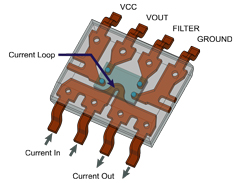
\includegraphics[width=0.5\linewidth]{ACS712.jpg}
\end{center}
\caption{Vhodni podatki.}\label{slika:acs}
\end{figure}

Senzor obstaja v treh različicah in sicer:

\begin{itemize}
\item ACS712ELCTR-05B-T
\item ACS712ELCTR-20A-T
\item ACS712ELCTR-30A-T
\end{itemize}

Razlikujejo se v občutljivosti oziroma koliko voltov razlike dobimo na izhodu za vsak izmerjen amper na vhodu, kar vpliva na to, kakšen je maksimalen tok ki ga lahko izmerimo. Kot je iz imen senzorjev razvidno so senzorji primerni za toke do 5A(185mV/a), 20A(100mV/A) in 30A(66mV/A) kot si sledijo.


SLIKA MOJIH SENZORJEV

Senzorji, ki smo jih uporabili za izdelavo prototipa smo kupili v obliki modulov(zgoraj omenjen senzor, z vsop otrebno periferijo za takojšnji priklop in uporabo). Senzorji imajo sicer sponko za priklop porabnika, vendar je merjenje vseeno indirektno, saj je senzor galvansko ločen. Zaradi potrebe po reaznju žice porabnika, za priklop senzorja, ta oblika senzorja ni najbolj optimalna za končni izdelek, za izdelavo prototipa pa bo zadostovala.

SLIKA PRIMERNEJŠEGA SENZORJA.

\section{RMS - Root mean square}

Za določeno število vrednosti n diskretne porazdelitve xi, ..., xn, root mean square (krajše RMS, včasih imenovan tudi
quadratic mean), je kvadratni koren povprečja vrednosti vseh xi na kvadrat.

FORMULA

Zgornji izračun lahko nekoliko poenostavimo, če vemo da je signal katerega želimo izračunati RMS vrednost, sinusoiden.
Periodična sinusoidna napetost je konstanten in je definiran kot V(t) = Vm*cos(wt) s periodo T. Tako lahko izračunamon RMS
vrednost sinusoidne napetosti V(t) kot

FORMULA

http://www.electronics-tutorials.ws/accircuits/rms-voltage.html
http://mathworld.wolfram.com/Root-Mean-Square.html


\section{Merjenje izmeničnega toka s senzorjem}
Eden od problemov pri merjenu izmeničnega toka je ta, da senzor meri samo trenutno vrednost. Ker je merjeni signal(izmenični) sinusne oblike, to pomeni da bi lahko za enak porabnik, izmeril več različnih vrednosti, odvisno od časa opravljene meritve.

SLIKA SINUSA Z OZNAČENIMI MERITVAMI KI KAŽEJO DRUGAČNE VREDNOSTI.

Za točno meritev moremo torej s pomočjo meritev izračunati RMS(root mean square) vrednost. Za izračun RMS potrebujemo maksimalno in minimalno vrednost merjenega signala. Ker ima izmenični tok frekvenco 50Hz, moramo opraviti meritve dovolj pogosto, da bomo pridobili čim bolj točne vrednosti. Z maksimalno in minimalno vrednostjo, lahko izračunamo VPP(Volts peak to peak). Dobljeno vrednost nato delimo z 2, da dobimo VPK(Volts peak), katero nato delimo s korenom od 2, da dobimo RMS vrednost sinusnega signala. Dobljena vrednost je sedaj naša želena merjena vrednostizmeničnega toka.

SLIKA ENAČBE

SLIKA KODE IN OBRAZLOŽITEV.



\chapter{Načrtovanje aplikacije}

\section{HTTP protokol}
The Hypertext Transfer Protocol (HTTP) is an application-level
   protocol for distributed, collaborative, hypermedia information
   systems. HTTP has been in use by the World-Wide Web global
   information initiative since 1990. The first version of HTTP,
   referred to as HTTP/0.9, was a simple protocol for raw data transfer
   across the Internet. HTTP/1.0, as defined by RFC 1945 [6], improved
   the protocol by allowing messages to be in the format of MIME-like
   messages, containing metainformation about the data transferred and
   modifiers on the request/response semantics. Dandanes se uporablja
   HTTP/1.1, ponekod tudi HTTP/2. 

   HTTP defines methods (sometimes referred to as verbs) to indicate the desired action to be performed on the identified resource. What this resource represents, whether pre-existing data or data that is generated dynamically, depends on the implementation of the server. Often, the resource corresponds to a file or the output of an executable residing on the server. The HTTP/1.0 specification[11] defined the GET, POST and HEAD methods and the HTTP/1.1 specification[12] added 5 new methods: OPTIONS, PUT, DELETE, TRACE and CONNECT. By being specified in these documents their semantics are well known and can be depended on. Any client can use any method and the server can be configured to support any combination of methods. If a method is unknown to an intermediate it will be treated as an unsafe and non-idempotent method. There is no limit to the number of methods that can be defined and this allows for future methods to be specified without breaking existing infrastructure. For example, WebDAV defined 7 new methods and RFC 5789 specified the PATCH method.


GET
The GET method requests a representation of the specified resource. Requests using GET should only retrieve data and should have no other effect. (This is also true of some other HTTP methods.)[1] The W3C has published guidance principles on this distinction, saying, "Web application design should be informed by the above principles, but also by the relevant limitations."[13] See safe methods below.
HEAD
The HEAD method asks for a response identical to that of a GET request, but without the response body. This is useful for retrieving meta-information written in response headers, without having to transport the entire content.
POST
The POST method requests that the server accept the entity enclosed in the request as a new subordinate of the web resource identified by the URI. The data POSTed might be, for example, an annotation for existing resources; a message for a bulletin board, newsgroup, mailing list, or comment thread; a block of data that is the result of submitting a web form to a data-handling process; or an item to add to a database.[14]
PUT
The PUT method requests that the enclosed entity be stored under the supplied URI. If the URI refers to an already existing resource, it is modified; if the URI does not point to an existing resource, then the server can create the resource with that URI.[15]
DELETE
The DELETE method deletes the specified resource.
TRACE
The TRACE method echoes the received request so that a client can see what (if any) changes or additions have been made by intermediate servers.
OPTIONS
The OPTIONS method returns the HTTP methods that the server supports for the specified URL. This can be used to check the functionality of a web server by requesting '*' instead of a specific resource.
CONNECT
[16] The CONNECT method converts the request connection to a transparent TCP/IP tunnel, usually to facilitate SSL-encrypted communication (HTTPS) through an unencrypted HTTP proxy.[17][18] See HTTP CONNECT tunneling.
PATCH
The PATCH method applies partial modifications to a resource.[19]
All general-purpose HTTP servers are required to implement at least the GET and HEAD methods,[20] and, whenever possible, also the OPTIONS method.[citation needed]

https://tools.ietf.org/html/rfc2616


\section{Laravel framework}
Prva beta verzija Laravel 1 frameworka je bila napisana iz nič(od začetka??). in je bila izdana Junija 2011. Vsebovala je ORM(Eloquent) narejen po meri, closure-based routing, sistemski modul za extension in helpers za forme, validacijo, autentikacijo in več.

Zgodnji razvoj Laravel frameworka se je razvijal hitro. Laravel 2 in 3 sta bila izdana novembra 2011 in februarja 2012. Novosti v laravelu 2 in 3 so bili kontrolerji, unit testiranje, command line orodje, inversion of control(Ioc) container, Eloquent relacije in migracije.

Laravel 4 je bil ponovno napisan od nule(začetka???) in je bil izdan maja 2013 v novi strukturi, saj se je v tej točki composer(php's ubiquitous package manager) začel kazati za dober industrijski standard, kar je pokazalo velik potencijal za framework, napisan kot zbirka komponent, ki je bila povezana med seboj s strani kompozerja. Laravel je bil zato razvit kot zbirka komponent pod imenom Illuminate in od te točke naprej ni bil več na voljo kot download, ampak je uporabljal večino komponent od Symfony-ja(še en framework, ki dovoljuje uporabo komponent ostalim) in komponente Illuminate s pomočjo Composerja. Ker je laravel od tedaj naprej uporabljal veliko komponent symfony-ja, je prejemal 6 mesečne posodobitve, saj so sledili posodobitvam symfony-ja. Z izdajo Laravel 4 frameworka, so predstavili tudi vrste, mail komponente, facades, in database seeding.

Laravel 4.3 bi moral biti izdan novembra 2014, vendar so pri razvoju zaradi potrebe po velikih spremembah ugotovili, da ne bodo uspeli izdati nove verzije do omenjenega roka. Laravel 5 je bil zato izdan februarja 2015 z njim pa so prišle novosti kot so nova direktorna struktura, odstranitev helperjev za forme in html, introduction of the contract interfaces, a spate of new views, socialite for social media authentication, elixir for asset compilation, scheduler to simplify cron, dotenv for simplified enironmant management, form requests and a brand new repl(read evaluate print loop)


BOOK: LARAVEL UP AND RUNNING

\subsection{Zakaj Laravel}

Od vseh server-side programskih jezikov, je PHP eden od bolj popularnih. Nameščen je na veliki večini sistemov za web host in je tudi zelo enostaven za namestitev na osebne računalnike. PHP je dokaj enostaven, še posebej se znajdejo dobro začetniki, ki že imajo nekaj predhodnega znanja s htmljem, konceptom spremenljivk, inline conditions in include statementi. PHP ponuja tudi veliko pogosto uporabljenih funkcij, ki jih uporabljamo pri razvijanju spletnih strani. Seveda ima PHP zaradi svoje enostavnosti tudi nekaj drawbacks. Še posebej pri začetnikih, ki uporabljajo PHP velikokgrat pride do nepotrebne kompleksne kode, ki v večini primerov ni ločena po funkcionalnosti, saj nas nič ne prisili k temu. 

Velikokrat ko razvijamo aplikacije brez frameworka, imamo nekje spravljene že napise funkcije, katere pogosto uporabljamo za reševanje pogostih problemov kot so upravljanje s podatkovno bazo, autenticiranje uporabnokov... Problem pri tem je, da moramo sami skrbeti za vzdrževanje kode, kar lahko enostavno rešimo s frameworkom kot je laravel, saj nas med drugim prisili k ločevanju kode po funckionalnosti in skrbi za vzdrževanje že obstoječih funkcij.

BOOK: GETTING STARTED WITH LARAVEL

\subsection{Glavne funkcionalnosti}

\begin{itemize}
\item \textbf{Modularnost:} Laravel je bil zgrajen na več kot 20 različnih knjižnicah in je razdeljen v posamezne module. Ker je močno povezan z composer dependency managerjem, ga lahko zelo enostavno posodobimo.
\end{itemize}


\section{strežnik}

\section{baza}

\chapter{Izvedba}
\thispagestyle{fancy}
\pagenumbering{arabic}

\chapter{Testiranje}
\thispagestyle{fancy}
\pagenumbering{arabic}

\chapter{Zaključek}
\thispagestyle{fancy}
\pagenumbering{arabic}





\medskip
\noindent Zgled citiranja:

\medskip
Minimiziranje pasovnosti matrik pomaga pri njihovem shranjevanju in pri računanju z njimi, npr.~pri Gaussovi eliminaciji. Bralec bo podrobnosti našel v~\cite{Chinn, George, Strang}.


\chapter{Vložitve}
\thispagestyle{fancy}

Dodamo vezno besedilo.

\section{Široke vložitve}\label{siroke}

Dodamo vezno besedilo.

\subsection{Podpoglavje poglavja Široke vložitve}

Dodamo vezno besedilo.

\begin{defi}
Graf $G$ je {\em povezan}, če za vsaki dve točki $u,v\in V(G)$ obstaja vsaj ena $u$-$v$ pot v $G$.
\end{defi}

\begin{lema}
Lema je pomožna trditev, ki služi za dokaz glavnega izreka.
\end{lema}

\begin{proof}
Tu napišimo dokaz leme. Dokaz naj bo čim krajši, vendar razumljiv vsem študentom. Pazite na logično strukturo dokaza: Vsi koraki naj bodo utemeljeni.
\end{proof}

\begin{izr}
Izrek je najpomemnejša trditev v poglavju. Izrekov naj bo čim manj, preostale trditve formuliramo kot leme ali kot trditve.
\end{izr}

\begin{proof}
Tu napišemo dokaz izreka.
\end{proof}

\begin{posl}
Posledica je ugotovitev, ki neposredno sledi iz glavnega izreka. Potrebuje le krajši dokaz (par vrstic). Če se ne da dokazati v par vrsticah, potem to ni več posledica, temveč lema ali trditev.
\end{posl}

\begin{prim}
Z zgledom osvetlimo lemo ali glavni izrek. Zgled je lahko protiprimer k veljavnosti izreka, če mu izpustimo kakšno od hipotez.
\end{prim}

\newpage
Takole se vstavlja slika:

\bigskip
\bigskip
\begin{figure}[h!]
\begin{center}
\includegraphics[width=0.5\linewidth]{graf.pdf}
\end{center}
\caption{Vhodni podatki.}\label{slika:podatki}
\end{figure}

\newpage
 Takole se vstavlja tabela.

\begin{table}[h!]
\caption{Algoritem PLOGBAND}
\label{tabela:algoritem}
\fbox{%
      \parbox{\linewidth}{%
{\noindent \bf Algoritem PLOGBAND:}
\vskip 5pt
\indent Podatka: {\obeylines \indent \indent graf $G = G(V,E)$ na $n$ vozliščih in z $m$ povezavami,
% \indent \indent nenegativno celo število $L$.}
\indent \indent $L \in \N$.}
\begin{enumerate}

\item Za $1 \le j \le L$ naj bodo $p_j$ približno enakomerno
(geometrijsko) razporejena števila med $1 - 1/\log\log n$ in $1/\log n$.
Tj., vsa razmerja $p_j/p_{j+1}$ naj bodo približno enaka. (Natančne
formule so v~razdelku \ref{siroke}, kjer je opisana vložitev naključnih podmnožic.)

\item Uredi vozlišča glede na naraščajoče vrednosti $h(v)$. Vozlišča z enakimi
vrednostmi $h$ uredi poljubno.

\item Vrni urejeni seznam vozlišč kot linearno ureditev.
\end{enumerate}
}}
\end{table}

\noindent Takole navedemo sliko ali tabelo:

\medskip
Vse, kar potrebujemo za konec dokaza, je povzeto v Tabeli~\ref{tabela:algoritem}.

\medskip
Za primer vhodih podatkov glej Sliko~\ref{slika:podatki}.

\medskip
\noindent Podobno lahko označimo in navajamo razdelke, poglavja, izreke, ipd.


\newpage
Takole lahko zapišemo psevdokodo algoritma:

\begin{algorithm}[h!]\label{algoritem1}
\Vhod{Realni matriki $A$ in $B$ velikosti $n\times n$.}
\Izhod{Matrika $C = A\cdot B$.}
\caption{Množenje matrik}
{
    \Za{$i = 1, \ldots, n$}
    {
        \Za{$j = 1, \ldots, n$}
        {
            $C[i,j]:= A[i,1]\cdot B[1,j];$

            \Za{$k = 2, \ldots, n$}
            {
                $C[i,j]:= C[i,j]+A[i,k]\cdot B[k,j]$;
            }
        }
    }
    \Ce{$n = 2$}
    {
       ne naredi nič
    }
}
\Vrni{$C$;}
\end{algorithm}


\chapter{Naslov poglavja}
\thispagestyle{fancy}

Takole citiramo spletne vire:~\cite{splet1,splet2,splet3}.\\
Takole citiramo članke, sprejete v objavo ali v tisku:~\cite{Novak,Novak2,Novak3,Novak4}.\\
Takole citiramo članke, poslane v objavo:~\cite{Novak5,Novak6}.

%%%%%%%%%%%%%%%%%%%%%%%%%%%%%%%%%% Zaključek %%%%%%%%%%%%%%%%%%%%%%%%%%%%%%%%%%%%%
\chapter{Zaključek}
\thispagestyle{fancy}

V nekaj stavkih na kratko povzamemo, kaj smo v nalogi obravnavali.
Po želji lahko navedemo še kakšne dodatne reference za bralca, ki bi ga zanimalo kaj več, ipd.


%%%%%%%%%%%%%%%%%%%%%%%%%%%%%%%% Literatura %%%%%%%%%%%%%%%%%%%%%%%%%%%%%%%%%

 \begin{thebibliography}{99}
\thispagestyle{fancy}

\bibitem{Blum}
  \clanekVRevijiVecAvtorjev
    {A.~Blum, G.~Konjevod}{R.~Ravi}
    {Semidefinite relaxations for minimum bandwidth and other vertex-ordering problems}
   {Theor.~Comp.~Sci.}{235}
   {2000}{25--42}

\bibitem{Bourgain}
  \clanekVRevijiEnAvtor
    {J.~Bourgain}
    {On Lipschitz embedding of finite metric spaces in Hilbert space}
   {Israel J.~Math}{52}
   {1985}{46--52}

\bibitem{Chinn}
  \clanekVRevijiVecAvtorjev
    {P.~Chinn, J.~Chv\'atalov\'a, A.~Dewdney}{N.~Gibbs}
    {The bandwidth problem for graphs and matrices -- a survey}
   {J.~Graph Theory}{6}
   {1982}{223--254}

\bibitem{Chvatalova}
\doktorskaDisertacija
    {J.~Chv\'atalov\'a}
    {On the bandwidth problem for graphs}
    {Ph.D.~dissertation, University of Waterloo, 1980}

\bibitem{Frankl}
  \clanekVRevijiVecAvtorjev
    {P.~Frankl}{H.~Maehara}
    {The Johnson-Lindenstrauss lemma and the sphericity of some graphs}
   {J.~Comb.~Theory, Ser.~B}{44}
   {1988}{355--362}

\bibitem{Feige}
  \clanekVRevijiEnAvtor
    {U.~Feige}
    {Approximating the bandwidth via volume respecting embeddings}
    {J.~Comp.~Syst.~Sci.}{60}
    {2000}{510--539}

\bibitem{George}
  \knjigaVecAvtorjev {A.~George}{J.~Liu}
   {Computer Solution of Large Positive Definite Systems}
    {Prentice-Hall, 1981}

\bibitem{Grotschel}
  \knjigaVecAvtorjev  {M.~Gr\"otschel, L.~Lov\'asz}{A.~Schrijver}
   {Geometric Algorithms and Combinatorial Optimization}
    {Springer-Verlag, Berlin, 1987}

\bibitem{Kleitman}
   \clanekVRevijiVecAvtorjev
     {D.~Kleitman}{R.~Vohra}
     {Computing the bandwidth of interval graphs}
     {SIAM J.~Discrete Math.}{3}
     {1990}{373--375}

\bibitem{Knuth}
  \knjigaEnAvtor     {D.~Knuth}
   {The Art of Computer Programming, Vol.~2, Seminumerical Algorithms}
    {Addison Wesley, Second Edition, 1981}

\bibitem{Lagarias}
\poglavjeVKnjigiEnAvtor
   {J.~Lagarias}
   {Point Lattices}
   {R.~Graham, M.~Gr\"otschel, L.~Lov\'asz (ur.)}
   {Handbook of Combinatorics, Volume~1}
   {MIT Press, 1995}
   {919--966}

\bibitem{Linial}
   \clanekVRevijiVecAvtorjev
     {N.~Linial, E.~London}{Y.~Rabinovich}
   {The geometry of graphs and some of its algorithmic applications}
     {Combinatorica}{15}
     {1995}{215--245}

\bibitem{Novak}
   \clanekVRevijiEnAvtorSprejetVObjavo
     {J.~Novak}
   {Polynomial approximation of rational manifolds. I}
     {J.~Abstract~Approximation}

\bibitem{Novak2}
   \clanekVRevijiEnAvtorVTisku
     {J.~Novak}
   {Polynomial approximation of rational manifolds. II}
     {J.~Abstract~Approximation}

\bibitem{Novak3}
   \clanekVRevijiVecAvtorjevSprejetVObjavo
     {J.~Novak}{M.~Novak}
   {Polynomial approximation of rational manifolds. III}
     {J.~Abstract~Approximation}

\bibitem{Novak4}
   \clanekVRevijiVecAvtorjevVTisku
     {J.~Novak}{M.~Novak}
   {Polynomial approximation of rational manifolds. IV}
     {J.~Abstract~Approximation}

\bibitem{Novak5}
   \clanekVRevijiEnAvtorPoslanVObjavo
     {J.~Novak}
   {Polynomial approximation of rational manifolds. V}
     {2014}

\bibitem{Novak6}
   \clanekVRevijiVecAvtorjevPoslanVObjavo
     {J.~Novak}{M.~Novak}
   {Polynomial approximation of rational manifolds. VI}
     {2014}

\bibitem{Santalo}
  \knjigaEnAvtor     {L.A.~Santalo}
   {Integral Geometry and Geometric Probability}
    {Encyclopedia of Mathematics and its Applications, Volume 1, Addison Wesley, 1976}

\bibitem{Saxe}
   \clanekVRevijiEnAvtor
     {J.~Saxe}
   {Dynamic programming algorithms for recognizing small-bandwidth graphs in polynomial time}
     {SIAM J.~Alg.~Meth.}{1}
     {1980}{363--369}

\bibitem{Strang}
  \knjigaEnAvtor     {G.~Strang}
   {Linear Algebra and its Applications, Third Edition}
    {Saunders College \hbox{Publishing}, Harcourt Brace Jovanovich College Publishers, 1988}

\bibitem{Unger}
\konferencniClanekEnAvtor
    {W.~Unger}
    {The complexity of the approximation of the bandwidth problem}
    {Proc.~39th Annual IEEE Symposium on Foundations of Computer Science}
    {1998}
    {82--91}

\bibitem{splet1}
\spletniVirBrezAvtorja
    {Miller--Rabin primality test}
    {\newline http://en.wikipedia.org/wiki/Miller/\%E2\%80\%93Rabin\_primality\_test}
    {25}{4}{2014}

\bibitem{splet2}
\spletniVirBrezAvtorjaZInstitucijo
    {The Converse of Wilson's Theorem}{The Oxford Math Center}
    {http://www.oxfordmathcenter.com/drupal7/node/382}
    {25}{4}{2014}

\bibitem{splet3}
\spletniVirZAvtorjem
    {T.~Tao}
    {Algebraic probability spaces}
    {http://terrytao.wordpress.com/}
    {4}{7}{2014}

% Ena vrstica mora biti tu prazna zaradi pravilnih navedb na strani, kjer so reference citirane.
\end{thebibliography}
\newpage

%%%%%%%%%%%%%%%%%%%%%%%%%%%%%%%%%%%% Priloge %%%%%%%%%%%%%%%%%%%%%%%%%%%%%%%%%%%%%
\pagestyle{fancyplain}
\vspace*{\fill}
     \begin{center}
          \bf{\Huge{Priloge}}
     \end{center}
\vspace*{\fill}
\thispagestyle{fancy}

\appendix
\thispagestyle{empty}
\pagenumbering{gobble}

\addtocontents{toc}{\setcounter{tocdepth}{-1}}
\appendices{A Naslov prve priloge}
\chapter{Naslov prve priloge}
\thispagestyle{empty}
Tu dodamo prvo prilogo.

% pozor:
% ukaz
% \thispagestyle{empty}
% mora biti prisoten na vsaki strani priloge (da se ne prikaže glava dokumenta)

\appendices{B Naslov druge priloge}
\chapter{Naslov druge priloge}
\thispagestyle{empty}
Tu dodamo drugo prilogo.

% Pozor:
% ukaz
% \thispagestyle{empty}
% mora biti prisoten na vsaki strani priloge (da se ne prikaže glava dokumenta)

\addtocontents{toc}{\setcounter{tocdepth}{2}}
\end{document}
